\chapter{Electromagnetic Induction}
\begin{itemize}
    \item \emph{Magnetic flux} is the \emph{product} of \emph{an area} and the component of \emph{magnetic flux density perpendicular} to that area.
    \item In other words, let \(A\) be an area in a uniform magnetic field, of flux density \(B_\perp\) perpendicular to \(A\). Then, the magnetic flux \(\Phi\) through \(A\) is
    \[\Phi=B_\perp A.\]
    \item The area \(A\) here is a \emph{vector}! When we flip it through \(\pi\) radians, the magnetic flux through it is now \(-\Phi=-B_\perp A\). 
    \item \emph{One weber} is the \emph{magnitude of magnetic flux} through an \emph{area of} \(1\text{m}^2\) when a \emph{magnetic field of} \(1\text{T}\) acts \emph{perpendicularly into} the area.
    \item \emph{Magnetic flux linkage} through a coil is defined as the \emph{product} of the \emph{number of turns} of the coil and the magnetic flux through each turn of the coil.
    \item The magnetic flux linkage through a coil of \(N\) turns is hence
    \[N\Phi=NB_\perp A.\]
    \item \emph{Faraday's Law of Electromagnetic Induction} states that the \emph{e.m.f. induced} is \emph{directly proportional} to the \emph{rate of change of magnetic flux linkage}.
    \item \emph{Lenz's Law} states that the \emph{direction of the induced e.m.f.} is such that it may produce \emph{an effect} that \emph{opposes the change} causing it.
    \item Lenz's Law is a consequence of conservation of energy. Mechanical work done to enable the change in magnetic flux linkage is converted into electrical energy.
    \item Faraday's and Lenz's Laws imply that the e.m.f generated is
    \[E=-(N\Phi)'=-(NB_\perp A)'.\]
    (The negative sign indicates that the induced e.m.f. opposes the change in magnetic flux linkage.)
    \begin{center}
        \includegraphics[width=0.4\textwidth,page=4]{../images/Lenz's-Law/Lenz's-Law.pdf}
        \includegraphics[width=0.45\textwidth,page=5]{../images/Lenz's-Law/Lenz's-Law.pdf}
        \includegraphics[width=0.4\textwidth,page=3]{../images/Lenz's-Law/Lenz's-Law.pdf}
        \captionsetup{type=figure}
        \caption[figure]{\ref{Lenz's Law} Examples of Lenz's Law in action.}
    \end{center}
    \item Motional e.m.f.: Suppose we have a circuit as shown in the bottom left of the following figure. Then, by Faraday's Law,
    \[\lvert E \rvert=\Phi'=BA'=Blv.\]
    \begin{center}
        \begin{minipage}{0.9\textwidth}
            \centering
            \raisebox{-0.5\height}{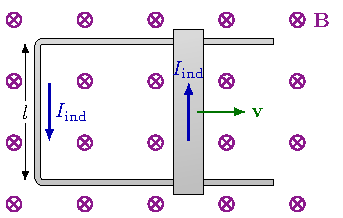
\includegraphics[width=0.58\textwidth,page=1]{../images/Lenz's-Law/Lenz's-Law.pdf}}
            \hspace*{.2in}
            \raisebox{-0.5\height}{\includegraphics[width=0.37\textwidth,page=2]{../images/Lenz's-Law/Lenz's-Law.pdf}}
            \captionsetup{type=figure}
            \caption[figure]{\ref{Lenz's Law} Example of motional emf.}
          \end{minipage}
    \end{center}
    \item Conventions for polarity and when to use them.
    \begin{center}
        \begin{tabular}{|Sc|Sc|Sc|}
            \hline
            Energy conversion & Function in a circuit & Convention for polarity\\
            \hline
            \textcolor{NavyBlue!80}{Electrical} to \textcolor{brown!70}{others} & Resistor/Wire & Higher potential\({}={}\)relatively positive\\
            \hline
            \textcolor{brown!70}{Others} to \textcolor{NavyBlue!80}{electrical} & Battery & Lower potential\({}={}\)relatively positive\\
            \hline
        \end{tabular}
    \end{center}
    \item Faraday's Paradox. Consider a metal disc with of area \(A\) rotating at frequency \(f\) in a uniform magnetic field, of flux density \(B\). Then, let \(\text{O}\) be the centre of the disk, and pick any point \(P\) along the circumference of the disk. We see that \(A'\), the area swept by \(\text{OP}\) per unit time, is \(\pi r^2f\). So, by Faraday's Law,
    \[E=B\pi r^2f.\]
    \begin{center}
        \includegraphics[width=0.4\textwidth]{../images/Faraday’s-Paradox.png}
        \captionsetup{type=figure}
        \caption[figure]{\ref{Me} An illustration of Faraday's Paradox.}
    \end{center}
    \begin{example}{}{}
        Initially, the switch is open. The switch is then closed for a short time and then reopened. Use Faraday's law of electromagnetic induction to explain what happens to the reading on the voltmeter. \hspace*{\fill} [5]
        \begin{figure}[H]
            \centering
            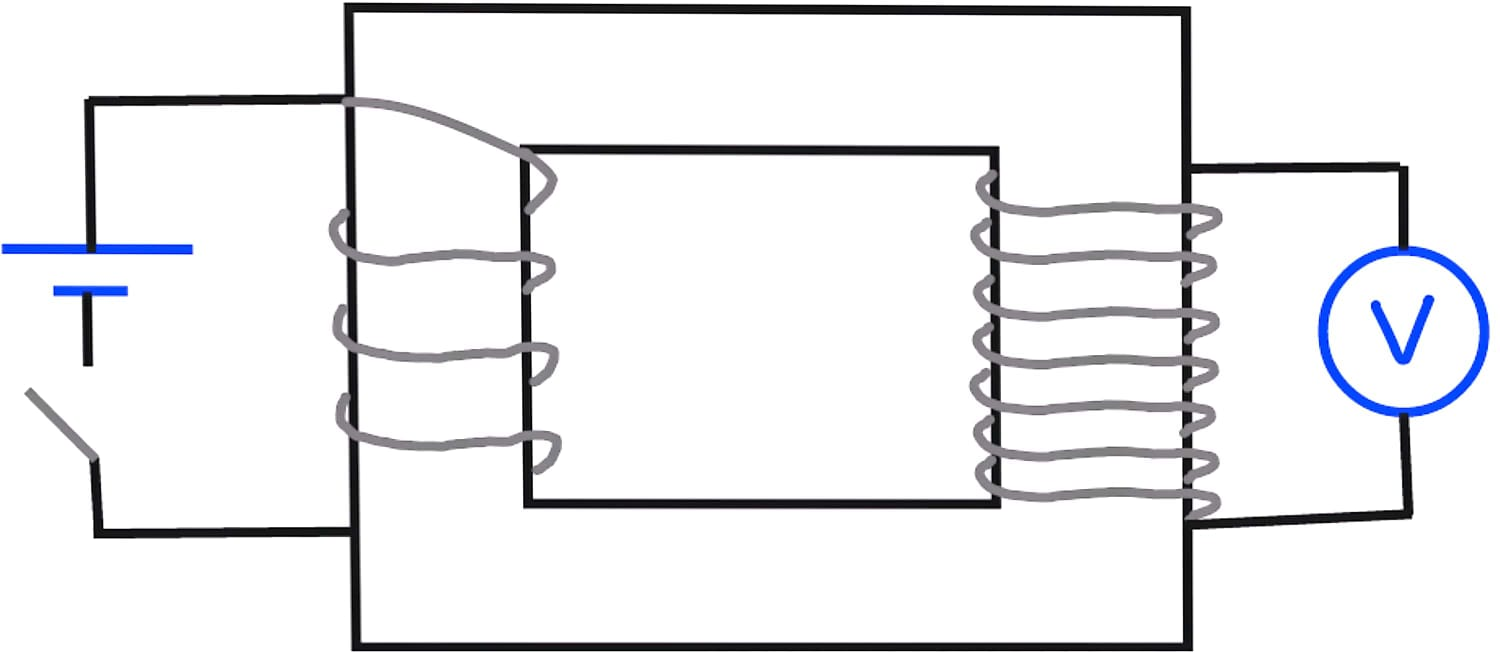
\includegraphics[width=0.5\textwidth]{../images/2022-transformer.jpg}
            \caption{\ref{Me}}
            \label{fig:2022-transformer}
        \end{figure}
        \begin{itemize}
            \item When the switch is closed for a short time, the circuit is closed and current flows through the primary coil. This causes the magnetic flux density in the primary coil (and hence the core) to increase. \hspace*{\fill} [1]
            \item The magnetic field is directed to the secondary coil by the iron core. \hspace*{\fill} [1]
            \item This causes the magnetic flux linkage through the secondary coil to increase. Hence, by Faraday's Law, e.m.f. is induced in the secondary coil; the the voltmeter registers a nonzero reading. \hspace*{\fill} [1]
            \item When the current in the primary coil reaches a constant value, the magnetic flux linkage through the secondary coil is constant. Thus, no e.m.f. is induced in the secondary coil. Accordingly, the voltmeter reading goes back to zero after a short time. \hspace*{\fill} [1]
            \item When the switch is re-opened, the decrease in current and magnetic flux density in the primary coil causes the magnetic flux linkage through the secondary coil to decrease; e.m.f. is again induced momentarily in the secondary coil, but in the opposite direction, before returning to zero \hspace*{\fill} [1].
        \end{itemize}
    \end{example}
    \item If asked to explain why an alternating current/e.m.f. is produced in the secondary coil, consider writing what follows. 
    
    \vspace{0.5\baselineskip} Since the rate of change of magnetic flux linkage alternates due to the alternating (sinusoidal) primary current, the induced e.m.f. in the secondary coil also alternates with the same frequency as the primary current.
    \begin{example}{}{}
        Assume that the transformer in the setup below is ideal.
        \begin{figure}[H]
            \centering
            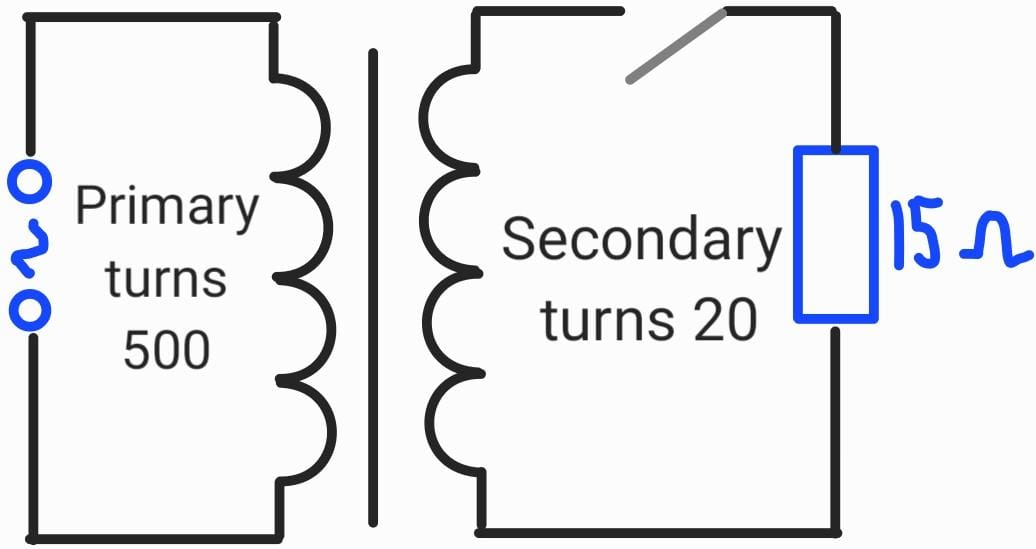
\includegraphics[width=0.5\textwidth]{../images/transformer-turns.jpg}
            \caption{\ref{Me}}
            \label{fig:transformer-step-down-emf-explanation}
        \end{figure}
        Use Faraday's law of electromagnetic induction to explain why the e.m.f. is less than the potential difference across the primary coil. 
        \begin{itemize}
            \item The soft-iron core provides a closed magnetic circuit which ensures that both the primary and secondary coils experience the same changing magnetic flux \(\Phi\).
            \item Since the secondary coil has a lower number of turns \(N\), by Faraday's Law, induced e.m.f 
            \[E=\frac{d(N\Phi)}{dt}=N \frac{d\Phi}{dt}\]
            is smaller for the secondary coil.
        \end{itemize}
    \end{example}
\end{itemize}